\chapter{Background}\label{chap:background}
This chapter provides an overview of the basic concepts of object detection and tracking and the steps of an Multi-Target Multi-Camera Tracking (MTMCT) system, along with a discussion of its key challenges and issues. Also the foundational building blocks of MTMCT are introduced. Futhermore it explains the datasets and metrics used to evaluate MTMCT systems.

\section{Steps of an MTMCT System}\label{sec:steps_of_an_mtmct_system}
An MTMCT system typically consists of the following steps: detection, feature extraction, data association, and tracking. Only the basic and fundamental concepts are explained in this section, more advanced and recent methods, mostly revolving around deep learning, will be discussed in chapter~\ref{chap:literature_review}.

\subsection{Detection}\label{subsec:detection}
Detection refers to the process of identifying objects of interest within video frames. This is typically done using a variety of techniques, ranging from traditional image processing methods to deep learning models. The objective of the detection step is to locate and classify objects in the frame, providing a basis for subsequent steps in the MTMCT process.

\subsection{Feature Extraction}\label{subsec:feature_extraction}
Feature extraction involves extracting relevant information from detected objects to facilitate tracking. This could include low-level features like color, shape and texture as well as high-level features like object parts and their spatial relationships, speed, and direction of movement. The features extracted from objects are used to identify and distinguish them from other objects in the scene.

\subsection{Data Association}\label{subsec:data_association}
To understand the data association step the following terms need to be defined:

\begin{itemize}
    \item \textbf{Tracklets:} Short segments of a path of an object captured within the view of a single camera, formed by connecting successive frame detections.
    \item \textbf{Trajectories:} The complete path of an object over time, often across multiple frames and cameras, created by merging together tracklets.
    \item \textbf{Tracks:} Refined trajectories that represent the validated path of an object after correction for inaccuracies and false detections.
\end{itemize}

In the research literature, these terms are often used interchangeably and not always consistently, but for the purposes of this project, the above definitions are used.

Data association is the process of associating current detected objects with existing tracks based on similarities in their features. This is done by comparing the features of detected objects with the features of existing tracks and assigning the detected objects to the most similar tracks. This step is critical in maintaining the identity of objects as they move through the scene or even leaving and re-entering the scene, which is called re-identification (re-ID). Commonly the data association step is first performed in a hierarchical manner: first on a single camera view (intra-camera), before the tracks are associated across multiple camera views (inter-camera) and finally being optimized globally.

\begin{figure}[ht]
    \centering
    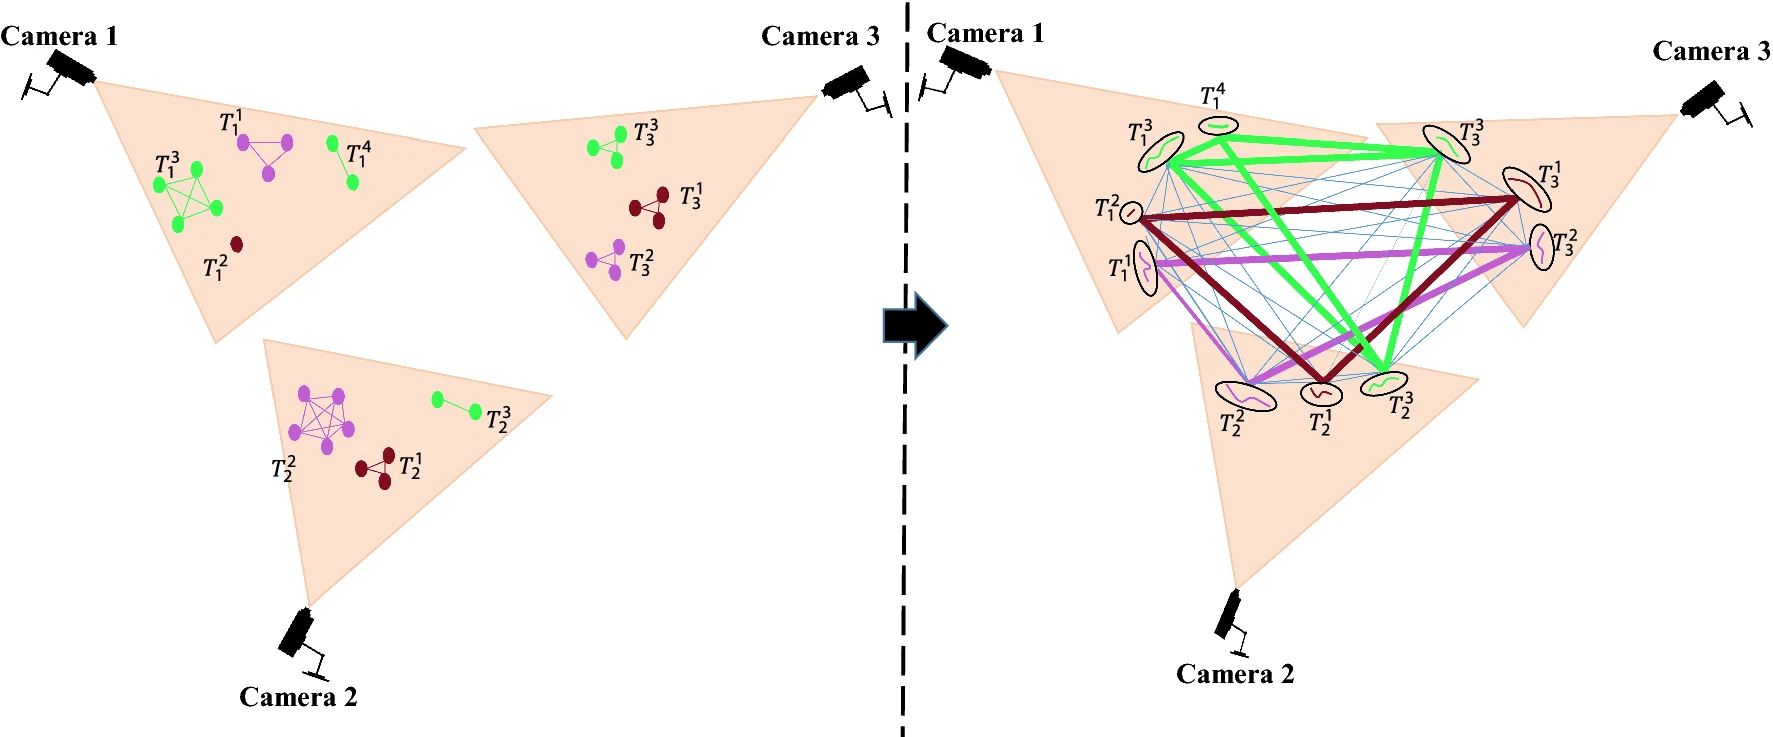
\includegraphics[width=0.75\textwidth]{resources/fig/Tesfaye19-intra_inter_camera_tracking.png}
    \caption{Intra- (left) and inter-camera (right) tracking~\cite[Fig.~1]{Tesfaye19}}\label{fig:intra_inter_camera_tracking}
\end{figure}

The two steps of data association of three non-overlapping camera views are illustrated in Figure~\ref{fig:intra_inter_camera_tracking}. The first step is intra-camera tracking, where the tracks are associated independently within the three camera views. The second step is inter-camera tracking, where the tracks are associated across the three camera views and the IDs of the objects are maintained. This simple example can be extended to any number of camera views, overlapping or non-overlapping.

\subsection{Tracking}\label{subsec:tracking}
Tracking refers to the step of maintaining the trajectory of detected objects over time. This involves predicting the future location of an object based on its past movements and updating its trajectory as new observations, so the next frame of a video, become available. To sum it up tracking is responsible for maintaining and managing the tracks and IDs of objects as they move through the scene and to ensure consistent global IDs across multiple camera views.

\section{Fundamental Concepts}\label{sec:fundamental_concepts}
This section briefly describes the preliminary concepts of MTMCT, which are essential to follow the progression from basic object tracking methods to advanced MTMCT techniques.

\subsection{Single-Target Single-Camera Tracking}\label{subsec:st_sct}
Single-Target Single-Camera Tracking (ST-SCT) is the simplest form of object tracking and involves tracking a single target in the field of view of a single camera. The primary goal of ST-SCT is to maintain the identity (ID) and trajectory of the target as it moves through the view of the camera.

\subsection{Multi-Target Single-Camera Tracking}\label{subsec:mt_sct}
Multi-Target Single-Camera Tracking (MT-SCT) builds upon the principles of ST-SCT but introduces the added complexity of dealing with multiple targets in a view of a single-camera. It aims to track multiple objects simultaneously while maintaining the ID of each target and avoiding ID switches. This requires sophisticated algorithms that can handle occlusions, interactions between targets, and other challenges that especially arise in crowded scenes.

The progression from ST-SCT to MT-SCT, and ultimately to MTMCT, reflects the increasing complexity and capability of tracking systems to handle more complex scenarios. This evolution is possible, due to advances in computer vision and machine learning, which provide the tools necessary to tackle the challenges associated with tracking multiple targets across multiple camera views.

\section{Challenges and Issues}\label{sec:challenges_and_issues}
The process of tracking multiple objects across various camera views requires careful consideration of various factors that can significantly affect the performance and accuracy of the tracking system. Some of the main challenges and issues faced in MTMCT are discussed in the following sections.

\subsection{Occlusion}\label{subsec:occlusion}
Occlusion occurs when an object is partially or completely blocked from view, making it difficult to accurately track its position and identity. This can happen when objects overlap with each other or are obstructed by other elements in the scene, such as buildings or trees. Occlusion is a common challenge in crowded environments, such as public spaces and sporting events, where multiple objects are often in close proximity to each other.

\subsection{Varying Lighting Conditions}\label{subsec:varying_lighting_conditions}
Lighting conditions can have a significant impact on the performance of an MTMCT system. Variations in lighting, such as changes in natural light throughout the day or artificial lighting when a tracked object enters a building, can affect the appearance of objects and make it challenging to maintain consistent tracking. The presence of shadows and reflections can also complicate the tracking process.

\subsection{Camera Specifications}\label{subsec:camera_specification}
The specifications of the cameras used in an MTMCT system can have a significant impact on its performance. When multiple cameras are used, they may have different:

\begin{itemize}
    \item \textbf{Resolution:} The number of pixels in the image
    \item \textbf{Frame rate:} The number of frames captured per second
    \item \textbf{Field of view (FOV):} The area captured by the camera
    \item \textbf{Angle:} The angle from which the camera captures the scene
\end{itemize}

This can make it challenging to maintain consistent tracking across different camera views, especially when objects move from one camera to another. Objects may appear differently when viewed from different cameras, and their size and shape can be distorted. Achieving accurate tracking requires the system to account for these variations and correctly align objects across different camera views.

\subsection{Uncertainties}\label{subsec:uncertainties}
In a MTMCT system, the number of present objects in the entire camera network, in a single camera view, and the number of camera views in which a tracked object is present at a given time are all unknown. This uncertainty complicates the precise tracking of objects across multiple camera views.

\section{Datasets}\label{sec:datasets}
Datasets are a fundamental aspect of MTMCT research, they are the resource for the training, evaluation, and comparison of various tracking methods. A diverse array of datasets exists to fullfil requirements of MTMCT research, each offering unique challenges and scenarios.

Commonly utilized datasets to train object detectors are:

\begin{itemize}
    \item \textbf{Microsoft COCO (Common Objects in Context):} Comprehensive dataset utilized for object detection, segmentation, and captioning. COCO comprises a diverse range of objects~\cite{Lin14}.
    \item \textbf{ImageNet:} Vast dataset employed for image classification and object detection. Object detectors trained on ImageNet are able to recognize an broad range of objects~\cite{Deng09}.
\end{itemize}

Beside these datasets, there are several datasets specifically designed for MTMCT research. These datasets are discussed in subsection~\ref{subsec:datasets_and_challenges}.

\section{Metrics and Evaluation}\label{sec:metrics_and_evaluation}
Evaluating the performance of a MTMCT system is critical to understand its effectiveness and reliability. Beside well known metrics like accuracy, precision and recall, there are several metrics specifically designed for multi-target and multi-camera systems. These metrics are discussed in the this section.

\subsection{MOTP and MOTA}\label{subsec:motp_mota}
The Multiple Object Tracking Precision (MOTP) and Multiple Object Tracking Accuracy (MOTA) are two standard metrics used for evaluating multi-target tracking systems. MOTP measures the accuracy of the object localization, while MOTA combines three types of errors into a single metric to provide a comprehensive evaluation of the tracking performance. Both of these metrics were introduced by \textcite{Bernardin08} in \citeyear{Bernardin08}.

\begin{equation}
    \label{eq:motp}
    \text{MOTP}=\frac{\sum_{i, t} d_t^i}{\sum_t c_t}
    \quad\text{\cite[Eq.~1]{Bernardin08}}
\end{equation}

Equation \ref{eq:motp} provides a measure of the average error in estimated positions of the tracked objects. In this equation, \(d_t^i\) represents the distance between the predicted position and the ground truth position of object \(i\) at frame \(t\), and \(c_t\) is the number of correctly matched objects (the true positives) in frame \(t\). The distances for all matched objects across all frames is divided by the total number of matched objects across all frames. MOTP ranges from 0 to 1, a lower MOTP value indicates higher precision in the object localization.

\begin{equation}
    \label{eq:mota}
    \text{MOTA}=1-\frac{\sum_t (m_t+fp_t+mme_t)}{\sum_t g_t}
    \quad\text{\cite[Eq.~2]{Bernardin08}}
\end{equation}

Equation \ref{eq:mota} combines three types of errors to give a single performance measure. In this equation, \(m_t\) is the number of misses (true objects not detected), \(fp_t\) is the number of false positives (spurious object detections), \(mme_t\) is the number of mismatch errors (identity switches) and \(g_t\) is the total number of true objects present in frame \(t\). The MOTA score is 1 minus the sum of all errors divided by the total number of true objects across all frames. MOTA ranges from \(-\infty\) to 1, a higher MOTA value indicates better tracking accuracy.

\subsection{IDF1}\label{subsec:idf1}
The IDF1 score is another important metric for evaluating MTMCT systems. It represents the harmonic mean of the identification precision and recall, providing a balanced measure that accounts for both the ratio of correctly identified detections and the average number of ground-truth and computed detections. This metric was introduced by \citeauthor{Ristani16} in their widely referenced paper \citetitle{Ristani16}~\cite{Ristani16}.

\begin{equation}
    \label{eq:idf1}
    \text{IDF}_1 = \frac{2 \times \text{IDTP}}{2 \times \text{IDTP} + \text{IDFP} + \text{IDFN}}
    \quad\text{\cite[Eq.~11]{Ristani16}}
\end{equation}

In equation~\ref{eq:idf1}:

\begin{itemize}
    \item \textbf{IDTP (Identification True Positives)}: Represents the number of detections that were correctly identified.
    \item \textbf{IDFP (Identification False Positives)}: Denotes the number of detections that were wrongly identified (misidentifications).
    \item \textbf{IDFN (Identification False Negatives)}: Indicates the number of actual detections that were missed or not identified.
\end{itemize}

The IDF1 metric essentially captures the identification precision and recall in multi-object tracking scenarios. The higher the IDF1 score, the better the performance of the tracker in maintaining consistent identities.

\subsection{MT and ML}\label{subsec:mt_ml}
The Mostly Tracked (ML) and Mostly Lost (ML) are used to assess the effectiveness of a tracking system in maintaining consistent trajectories for the objects being tracked. The metrics published by \textcite{Wu06} in \citeyear{Wu06} are commonly used in the MOTChallenge benchmarks to evaluate the performance of tracking systems.

MT measures the proportion of ground truth trajectories that are covered by the tracker for at least 80\% of their respective lifetimes, indicating the ability of the system to consistently track objects over time. On the other hand, ML measures the proportion of ground truth trajectories that are covered by the tracker for less than 20\% of their respective lifetimes, reflecting the inability of the system to maintain consistent object tracking.

\begin{figure}[ht]
    \centering
    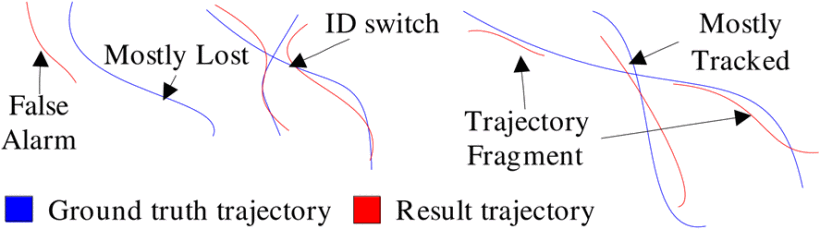
\includegraphics[width=0.75\textwidth]{resources/fig/Wu06-MT_ML.png}
    \caption{MT and ML~\cite[Fig.~5]{Wu06}}\label{fig:mt_ml}
\end{figure}

Figure~\ref{fig:mt_ml} illustrates various scenarios encountered in multi-target tracking evaluations:

\begin{itemize}
    \item \textbf{Ground Truth Trajectory (Blue):} Represents the actual path or movement of an object in the scene.
    \item \textbf{Result Trajectory (Red):} Represents the predicted path of an object by the tracking system.
    \item \textbf{False Alarm:} Points where the tracking system detects an object when there is no one present in the ground truth.
    \item \textbf{ID Switch:} An instance where the tracking ID assigned to an object changes erroneously during tracking.
    \item \textbf{Trajectory Fragment:} A segment of the result trajectory that is shorter than the ground truth, indicating a break or interruption in tracking.
    \item \textbf{Mostly Tracked:} Scenarios where the result trajectory closely follows the ground truth trajectory for the majority of the path of the object (\(\geq 80\%\))
    \item \textbf{Mostly Lost:} Scenarios where the result trajectory only briefly aligns or intersects with the ground truth trajectory, indicating the object was not effectively tracked for most of its path (\(\leq 20\%\)).
\end{itemize}